% Isto é um exemplo de Folha de aprovação, elemento obrigatório da NBR
% 14724/2011 (seção 4.2.1.3). Você pode utilizar este modelo até a aprovação
% do trabalho. Após isso, substitua todo o conteúdo deste arquivo por uma
% imagem da página assinada pela banca com o comando abaixo:
%
\begin{folhadeaprovacao}
    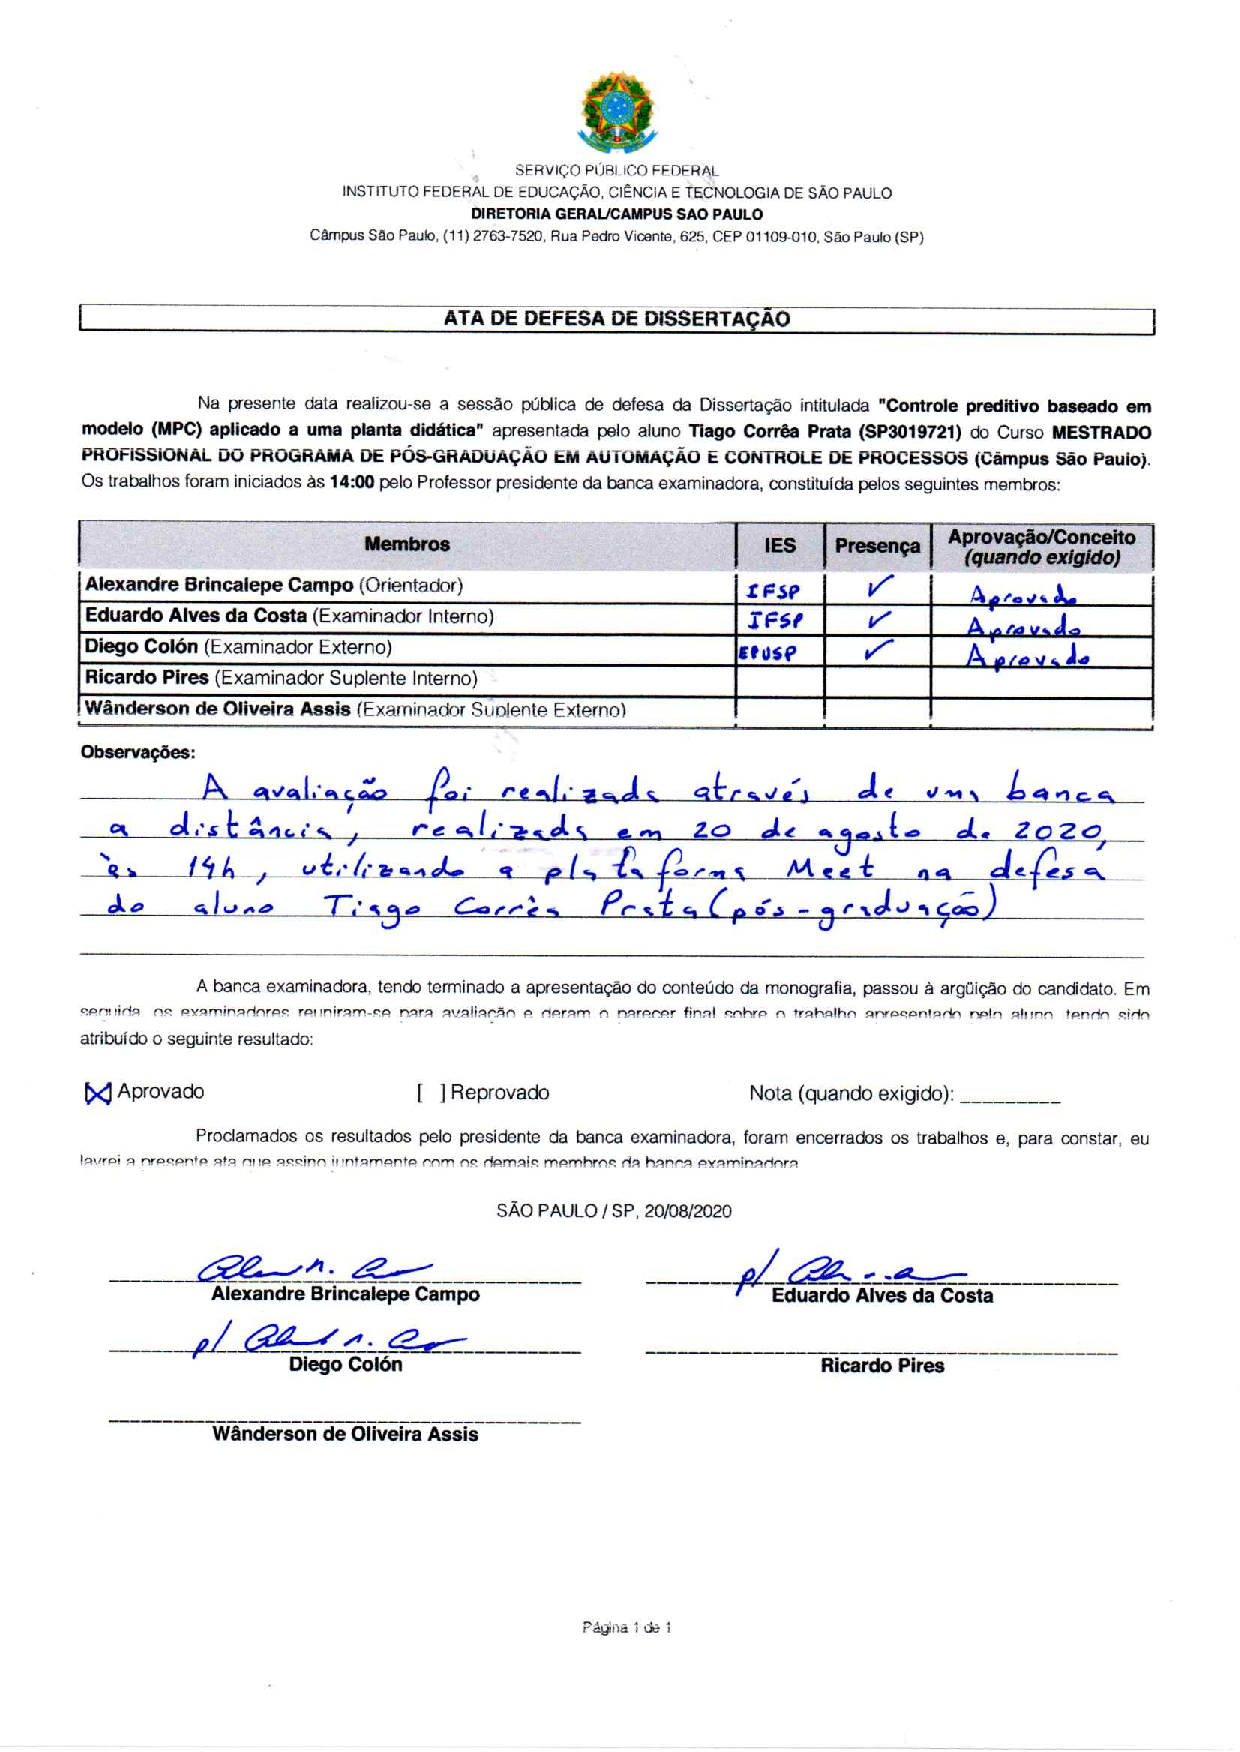
\includepdf{./1_pretext/folhaDeAprovacao_final.pdf}
\end{folhadeaprovacao}
%
% \begin{folhadeaprovacao}

%   \begin{center}
%     {\ABNTEXchapterfont\large\imprimirautor}

%     \vspace*{\fill}\vspace*{\fill}
%     \begin{center}
%       \ABNTEXchapterfont\bfseries\Large\imprimirtitulo
%     \end{center}
%     \vspace*{\fill}
    
%     \hspace{.45\textwidth}
%     \begin{minipage}{.5\textwidth}
%         \imprimirpreambulo
%     \end{minipage}%
%     \vspace*{\fill}
%    \end{center}
        
%    Trabalho aprovado. \imprimirlocal, 20 de agosto de 2020:

%    \assinatura{\textbf{\imprimirorientador} \\ Orientador} 
%    \assinatura{\textbf{Prof. Dr. Eduardo Alves da Costa} \\ Convidado (interno)}
%    \assinatura{\textbf{Prof. Dr. Diego Colón} \\ Convidado (externo)}
%    \assinatura{\textbf{Prof. Dr. Ricardo Pires} \\ Suplente (interno)}
%    \assinatura{\textbf{Prof. Dr. Wânderson de Oliveira Assis} \\ Suplente (externo)}
      
%    \begin{center}
%     \vspace*{0.5cm}
%     {\large\imprimirlocal}
%     \par
%     {\large\imprimirdata}
%     \vspace*{1cm}
%   \end{center}
  
% \end{folhadeaprovacao}